\documentclass{article}

\usepackage[catalan]{babel}
\usepackage[utf8]{inputenc}
\usepackage{amsmath}
\usepackage{amssymb}
\usepackage{enumerate}
\usepackage{listingsutf8} 	% \lstinputlisting[]{}
\usepackage{graphicx}		% \includegraphics{}
\usepackage{braket}			% \set{}
\usepackage[all,cmtip]{xy}
\usepackage{hyperref}

\usepackage{geometry}
\geometry{a4paper, total={210mm, 297mm}, left=25mm, right=20mm, top=20mm, bottom=20mm}

\newtheorem{theorem}{Teorema}[section]
\newtheorem{proposition}[theorem]{Proposició}
\newtheorem{lemma}[theorem]{Lema}
\newtheorem{definition}[theorem]{Definició}
\newtheorem{example}[theorem]{Exemple}
\newtheorem{remark}[theorem]{Observació}

\newcommand{\N}{\mathbb{N}}
\newcommand{\Z}{\mathbb{Z}}
\newcommand{\Q}{\mathbb{Q}}
\newcommand{\R}{\mathbb{R}}
\newcommand{\C}{\mathbb{C}}
\newcommand{\ring}[1]{\mathcal{O}_{#1}}

\begin{document}

\title{Problem 12}
\author{Enric Florit Zacarías}
\date{23/12/2018}

\maketitle

\begin{enumerate}[a)]
\item Write a C function that, given a point $(x,y)$, computes $f(x,y)$ and $\nabla f(x,y)$.

The implementation is straightforward and can be found in the code. The gradient's components ($\frac{\partial f}{\partial x}$ and $\frac{\partial f}{\partial y}$) are computed separately, to find first points in section (b).

\item Compute a point on the curve (suggestion: compute an intersection of the curve with one of the coordinate axis.

We find this by means of the functions \texttt{first\_approx\_x} and \texttt{first\_approx\_y}, which in turn use the partial derivatives of $f$ and Newton's method by fixing $x=0$ and $y=0$. For instance, to find an approximation $(x,0)$, we iterate
$$x_{n+1}=x_n-\frac{f(x_n,0)}{\partial_x f(x_n,0)}$$
until $|f(x_{n+1},0)|<10^{-10}$, taking $x_0=0$. We reach the point $(0.326344025690, 0.0)$.


\item Suppose that we know $(x_0,y_0)$ such that $f(x_0, y_0)=0$. Write a C function that, given a suitable first guess, uses Newton method to find a zero of $f(x,y)$ at a distance $h$ from $(x_0,y_0)$. Note: consider the system of equations
	\begin{align*}
	f(x,y)&=0\\
	(x-x_0)^2 + (y-y_0)^2 &= h^2	
	\end{align*}

Set $g(x,y)=(x-x_0)^2+(y-y_0)^2-h^2$, we will use the function $H(x,y)=(f(x,y),g(x,y))$ to find the desired zero of $f$. Given a first guess $(x_1,y_1)$, we want to find $(\alpha,\beta)$ such that
$$0=H(\alpha,\beta)\approx H(x_1,y_1)+DH(x_1,y_1)\big((\alpha,\beta)-(x_1,y_1)\big)$$

by using a first order Taylor approximation. Now, solving for $(\alpha,\beta)$ we get
$$\alpha\approx (x_1,y_1)-\big(DH(x_1,y_1)\big)^{-1}H(x_1,y_1)$$

provided that $DH(x_1,y_1)$ is invertible. Let's compute the inverse: we have
$$DH(x,y)=\begin{pmatrix}\frac{\partial f}{\partial x} & \frac{\partial f}{\partial y}\\
	\frac{\partial g}{\partial x} & \frac{\partial g}{\partial y}\end{pmatrix}=
	\begin{pmatrix}\frac{\partial f}{\partial x} & \frac{\partial f}{\partial y}\\
	2(x-x_0) & 2(y-y_0)\end{pmatrix}$$
	
From here, its determinant is
$$|DH(x,y)|=2(y-y_0)\frac{\partial f}{\partial x} - 2(x-x_0)\frac{\partial f}{\partial y}$$

and finally the inverse we wanted is
$$\big(DH(x,y)\big)^{-1}=\frac{1}{2(y-y_0)\frac{\partial f}{\partial x} - 2(x-x_0)\frac{\partial f}{\partial y}}
\begin{pmatrix}
	2(y-y_0) & -\frac{\partial f}{\partial y}\\
	-2(x-x_0) & \frac{\partial f}{\partial x}
\end{pmatrix}.$$

Wrapping up, the program has to perform this operation (evaluating all partial derivatives at $(x_n,y_n)$):

$$(x_{n+1},y_{n+1})=(x_n,y_n)
-\frac{1}{2(y_n-y_0)\frac{\partial f}{\partial x} - 2(x_n-x_0)\frac{\partial f}{\partial y}}
\begin{pmatrix}
	2(y_n-y_0) & -\frac{\partial f}{\partial y}\\
	-2(x_n-x_0) & \frac{\partial f}{\partial x}
\end{pmatrix}
\begin{pmatrix}
	f(x_n,y_n)\\ 
	g(x_n,y_n)
\end{pmatrix}$$


\item Write a C progam to compute and write in a file a table of values of the (closed) curve $f(x,y)=0$, using as a distance between points the value $\delta=0.01$ (hint: use the unitary tangent vector to the curve at a given point to obtain a suitable first guess for the next point). All the points in the file have to satisfy that $|f(x,y)|<10^{-10}$. Use \texttt{gnuplot} to plot the curve.

We only have to combine the work done in (b) and (c), finding a proper approximation for the next iteration. To do this, notice that we are looking for a curve $(x(t),y(t))$ that satisfies 
$$f(x(t),y(t))=0,\ \forall t.$$

Differentiating with respect to $t$ we get
$$f_x(x,y)x'+f_y(x,y)y'=\langle(x,y),(f_x,f_y)\rangle=0$$
which means the tangent vector is normal to the gradient of the function at every $t$. Therefore, we may take as tangent vector either $tgt=(-f_y,f_x)$ or $-tgt$, dividing by its norm and multiplying by $\delta$. 

Finally, to make sure we ``don't go back along the curve", we compute the dot product of the last two tangent vectors. If $\langle tgt_{n+1},tgt_n\rangle<0$, we multiply $tgt_{n+1}$ by $-1$.

\[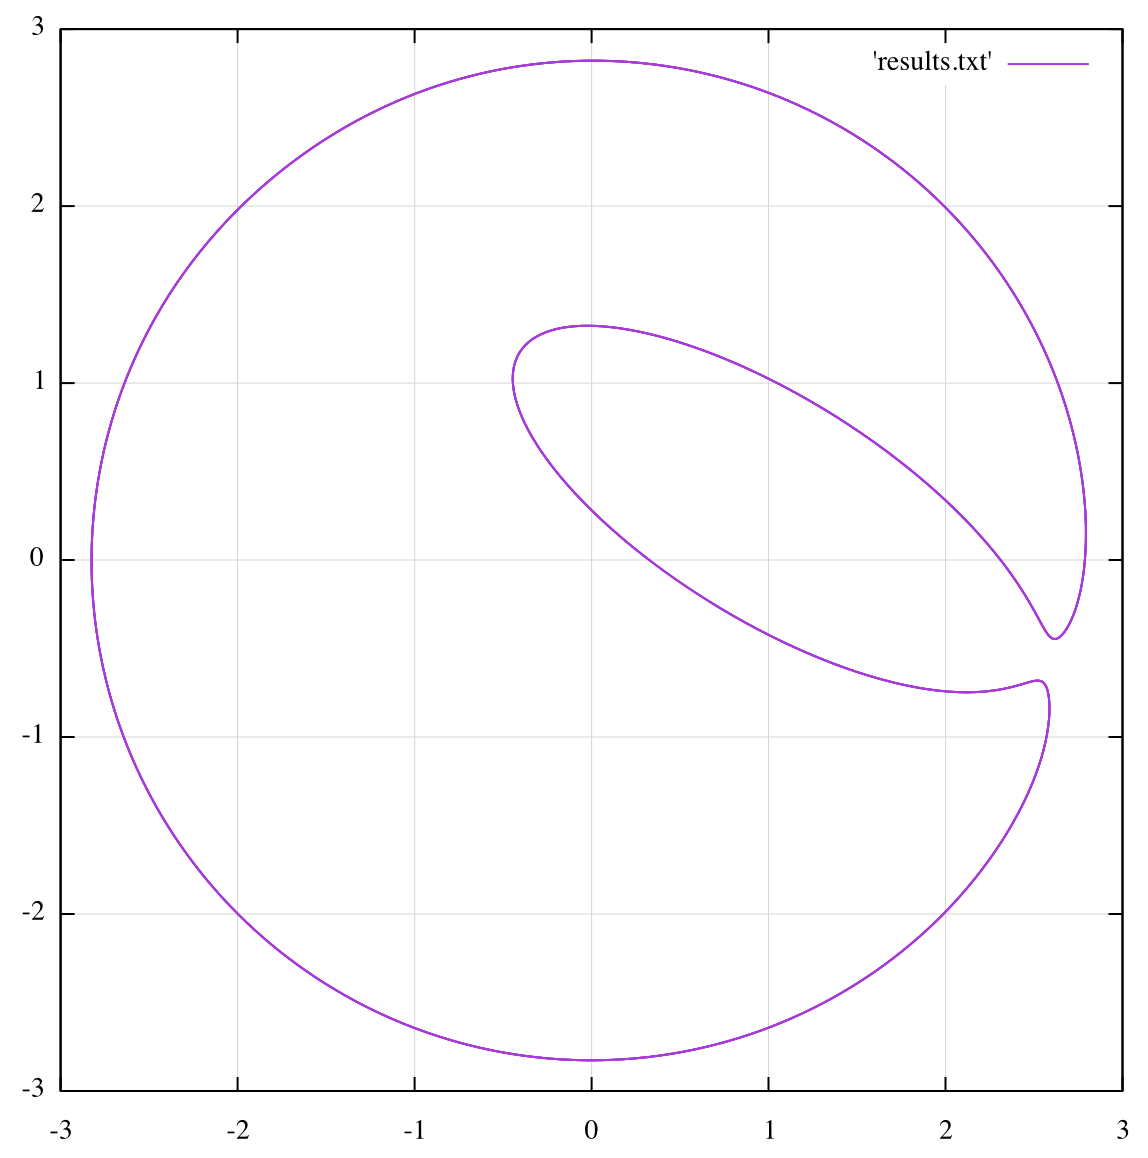
\includegraphics[width=0.6\textwidth]{plottedcurve}\]
\end{enumerate}




\end{document}
